\section{Experiments}
\subsection{Experimental Setup}
\paragraph{Datasets.} 
To evaluate the performance of \textsc{GraphSearch}, we conducted experiments on six multi-hop QA benchmarks within the RAG setting. The \textbf{Wikipedia}-based benchmarks include \textbf{HotpotQA}~\citep{hotpotqa}, \textbf{MuSiQue}~\citep{musique}, and \textbf{2WikiMultiHopQA}~\citep{2wiki} following~\citep{hipporag2, longfaith}. The \textbf{Domain}-based benchmarks~\citep{ultradomain} incorporate multi-hop questions synthesized by~\citep{hypergraphrag}, covering fields like \textbf{Medical}, \textbf{Agriculture}, and \textbf{Legal}. More details are provided in the Appendix~\ref{app:datasets}.

\begin{table*}[t]
\caption{Experiment results across six multi-hop QA benchmarks covering \textbf{Wikipedia}-based and \textbf{Domain}-based datasets. The + means \textbf{\textsc{GraphSearch}} integrates with various graph KB retrievers built upon the corresponding GraphRAG methods. The backbone LLM is \textit{Qwen2.5-32B-Instruct}.}
\label{Tab:main_exp}
\setlength{\tabcolsep}{4pt}
\begin{center}
% \small
\begin{tabular}{lccccccccc}
\toprule
\multirow{2}{*}{\normalsize\textbf{Method}}
& \multicolumn{3}{c}{\textbf{HotpotQA}}
& \multicolumn{3}{c}{\textbf{MuSiQue}}
& \multicolumn{3}{c}{\textbf{2WikiMultiHopQA}} \\
\cmidrule[1pt](lr){2-4} \cmidrule[1pt](lr){5-7} \cmidrule[1pt](lr){8-10}
& {\scriptsize $\mathrm{SubEM}$} & {\scriptsize $\mathrm{A\text{-}Score}$} & {\scriptsize $\mathrm{E\text{-}Score}$}
& {\scriptsize $\mathrm{SubEM}$} & {\scriptsize $\mathrm{A\text{-}Score}$} & {\scriptsize $\mathrm{E\text{-}Score}$}
& {\scriptsize $\mathrm{SubEM}$} & {\scriptsize $\mathrm{A\text{-}Score}$} & {\scriptsize $\mathrm{E\text{-}Score}$} \\
\midrule
Vanilla LLM      & 33.67 & 6.90 & 5.98 & 12.33 & 6.10 & 5.87 & 48.33 & 6.95 & 4.50 \\
Naive RAG        & 72.00 & 8.88 & 9.04 & 40.00 & 7.21 & 8.18 & 72.33 & 7.93 & 8.03 \\
ReAct            & 33.33 & -    & -    & 16.00 & -    & -    & 51.33  & -    & -    \\
\midrule
\multicolumn{10}{c}{\textbf{GraphRAG Baselines}} \\
\midrule
GraphRAG         & 72.67 & 8.18 & 8.65 & 36.67 & 6.58 & 7.32 & 79.33 & 7.44 & 7.99 \\
LightRAG         & 73.00 & 8.30 & 8.66 & 35.00 & 6.50 & 7.28 & 81.67 & 7.62 & 7.94 \\
MiniRAG          & 68.00 & 7.95 & 8.24 & 41.00 & 6.93 & 7.67 & 74.00 & 7.57 & 7.61 \\
PathRAG          & 79.00 & 8.99 & 9.17 & 46.33 & 7.26 & 8.02 & 77.00 & 8.25 & 8.34 \\
HippoRAG2        & 76.67 & 8.45 & 8.73 & 44.00 & 7.07 & 7.88 & 72.33 & 7.98 & 8.01 \\
HyperGraphRAG    & 74.33 & 7.39 & 8.69 & 41.67 & 6.76 & 7.53 & 64.00 & 7.62 & 7.80 \\
\midrule
\multicolumn{10}{c}{\textbf{\textsc{GraphSearch}}} \\
\midrule
\rowcolor{gray!20}
+ LightRAG       & 79.00 & 9.21 & \textbf{9.46} & 51.00 & 7.72 & 8.38 & 85.00 & 9.21 & 9.12 \\
\rowcolor{gray!20}
+ PathRAG        & \textbf{82.00} & \textbf{9.24} & 9.42 & \textbf{55.33} & \textbf{7.83} & \textbf{8.48} & \textbf{88.67} & \textbf{9.32} & \textbf{9.29} \\
\rowcolor{gray!20}
+ HyperGraphRAG  & 80.33 & 9.19 & 9.35 & 49.33 & 7.73 & 8.22 & 83.33 & 8.84 & 8.75 \\
\bottomrule
\toprule
\multirow{2}{*}{\normalsize\textbf{Method}}
& \multicolumn{3}{c}{\textbf{Medicine}}
& \multicolumn{3}{c}{\textbf{Agriculture}}
& \multicolumn{3}{c}{\textbf{Legal}} \\
\cmidrule[1pt](lr){2-4} \cmidrule[1pt](lr){5-7} \cmidrule[1pt](lr){8-10}
& {\scriptsize $\mathrm{SubEM}$} & {\scriptsize $\mathrm{A\text{-}Score}$} & {\scriptsize $\mathrm{E\text{-}Score}$}
& {\scriptsize $\mathrm{SubEM}$} & {\scriptsize $\mathrm{A\text{-}Score}$} & {\scriptsize $\mathrm{E\text{-}Score}$}
& {\scriptsize $\mathrm{SubEM}$} & {\scriptsize $\mathrm{A\text{-}Score}$} & {\scriptsize $\mathrm{E\text{-}Score}$} \\
\midrule
Vanilla LLM      & 21.29 & 7.14 & 7.57 & 29.88 & 7.10 & 7.38 & 37.11 & 7.02 & 7.43 \\
Naive RAG        & 54.34 & 8.23 & 8.67 & 54.24 & 7.91 & 8.26 & 53.36 & 7.37 & 7.67 \\
ReAct            & 19.73 & -    & -    & 25.99 & -    & -    & 30.86  & -    & -    \\
\midrule
\multicolumn{10}{c}{\textbf{GraphRAG Baselines}} \\
\midrule
GraphRAG         & 53.32 & 7.59 & 7.98 & 57.81 & 7.84 & 7.66 & 58.98 & 7.57 & 7.23 \\
LightRAG         & 49.80 & 7.36 & 7.57 & 55.66 & 7.38 & 7.32 & 56.84 & 7.01 & 6.78 \\
MiniRAG          & 56.84 & 8.13 & 8.51 & 59.38 & 8.08 & 8.08 & 61.91 & 7.70 & 7.50 \\
PathRAG          & 58.79 & 8.18 & 8.32 & 61.13 & 8.22 & 8.23 & 62.30 & 7.96 & 7.91 \\
HippoRAG2        & 55.08 & 7.90 & 8.03 & 58.20 & 7.95 & 7.86 & 64.45 & 8.02 & 7.81 \\
HyperGraphRAG    & 62.11 & 8.39 & 8.70 & 63.67 & 8.35 & 8.49 & 66.60 & 8.18 & 8.18 \\
\midrule
\multicolumn{10}{c}{\textbf{\textsc{GraphSearch}}} \\
\midrule
\rowcolor{gray!20}
+ LightRAG       & 65.88 & 8.61 & 8.80 & 63.53 & 8.52 & 8.48 & 71.68 & 8.45 & 8.52 \\
\rowcolor{gray!20}
+ PathRAG        & 70.12 & 8.59 & 8.82 & 69.34 & 8.63 & 8.78 & 74.41 & 8.32 & 8.49 \\
\rowcolor{gray!20}
+ HyperGraphRAG  & \textbf{73.24} & \textbf{8.87} & \textbf{9.24} & \textbf{73.83} & \textbf{8.93} & \textbf{9.02} & \textbf{78.52} & \textbf{8.76} & \textbf{8.83} \\
\bottomrule
\end{tabular}
\vspace{-20pt}
\end{center}
\end{table*}

\paragraph{Baselines.} 
We compare \textsc{GraphSearch} with several baseline methods, including \textbf{Vanilla LLM}, \textbf{Naive RAG}~\citep{rag}, \textbf{GraphRAG}~\citep{graphrag}, \textbf{LightRAG}~\citep{lightrag}, \textbf{MiniRAG}~\citep{minirag}, \textbf{PathRAG}~\cite{pathrag}, \textbf{HippoRAG2}~\citep{hipporag2}, and \textbf{HyperGraphRAG}~\citep{hypergraphrag}. More details are provided in the Appendix~\ref{app:baselines}.

\paragraph{Evaluation Metrics.} 
We adopt three evaluation metrics to assess the QA and retrieval quality of \textsc{GraphSearch} and baselines. The string-based Substring Exact-Match (\textbf{SubEM}) metric checks whether the golden answer is explicitly contained in the response. The Answer-Score (\textbf{A-Score}) covers \textbf{Correctness}, \textbf{Logical Coherence}, and \textbf{Comprehensiveness}. The Evidence-Score (\textbf{E-Score}) measures \textbf{Relevance}, \textbf{Knowledgeability}, and \textbf{Factuality}. Both A-Score and E-Score are assessed using the LLM-as-a-Judge~\citep{llm-as-a-judge}. More details are provided in the Appendix~\ref{app:evaluation}.

\subsection{Main Results}

\paragraph{\textsc{GraphSearch} outperforms all GraphRAG baselines.} 
\begin{wrapfigure}{r}{0.35\textwidth}
\vspace{-15pt}
\centering

\includegraphics[width=0.35\textwidth]{figs/radar.pdf}
\caption{Judge results across eight metrics on A-Score and E-Score.}
\label{fig:radar}
\vspace{-25pt}
\end{wrapfigure}
As shown in Table~\ref{Tab:main_exp}, comparing with GraphRAG methods that perform only a single round of graph retrieval and generation, \textsc{GraphSearch} leverages the constructed graph knowledge bases with the graph KB retriever to enable multi-turn interactions. Across six benchmarks covering Wikipedia and domain-based datasets, \textbf{\textsc{GraphSearch} achieves the best overall performance}. This confirms the importance of adopting an agentic workflow for deep searching over GraphRAG in complex reasoning scenarios, effectively mitigating the insufficiencies of vanilla strategies caused by limited interaction and inadequate retrieval. Case studies with more detail information of are provided in Figure~\ref{fig:case_baseline} and Figure~\ref{fig:case_graphsearch} in Appendix~\ref{app:case_study}.

\paragraph{\textsc{GraphSearch} exhibits strong plug-and-play capability.} 
As shown in Table~\ref{Tab:main_exp}, when applied with various retrieval methods over different graph KBs, \textsc{GraphSearch} consistently yields improvements compared to their native interaction schemes. For example, it boosts LightRAG on MuSiQue, raising SubEM from $\mathbf{35.00}$ to $\mathbf{51.00}$, while improving A-Score and E-Score from $\mathbf{6.50}$ and $\mathbf{7.28}$ to $\mathbf{7.72}$ and $\mathbf{8.38}$. Similarly, it enhances HyperGraphRAG on Medicine, increasing SubEM from $\mathbf{62.11}$ to $\mathbf{73.24}$, and further elevating A-Score and E-Score from $\mathbf{8.39}$ and $\mathbf{8.70}$ to $\mathbf{8.87}$ and $\mathbf{9.24}$. These results demonstrate the plug-and-play capability of \textsc{GraphSearch}, with detailed results presented in Figure~\ref{fig:radar}.


\subsection{Ablation Studies} 

\begin{wraptable}{r}{0.50\textwidth}
\vspace{-20pt}
\caption{Results across two benchmarks. The backbone LLM is \textit{Qwen2.5-7B-Instruct}.}
\label{Tab:ab_exp_7B}
\scriptsize
\setlength{\tabcolsep}{2pt}
\begin{center}
\begin{tabular}{lcccccc}
\toprule
\multirow{2}{*}{\textbf{Method}}
& \multicolumn{3}{c}{\textbf{2Wiki.}}
& \multicolumn{3}{c}{\textbf{Legal}} \\
\cmidrule[1pt](lr){2-4} \cmidrule[1pt](lr){5-7}
& {\scriptsize $\mathrm{SubEM}$} & {\scriptsize $\mathrm{A\text{-}S}$} & {\scriptsize $\mathrm{R\text{-}S}$}
& {\scriptsize $\mathrm{SubEM}$} & {\scriptsize $\mathrm{A\text{-}S}$} & {\scriptsize $\mathrm{R\text{-}S}$} \\
\midrule
Vanilla LLM      &  46.67 &  6.26 &  3.70 &  34.18 &  6.47 & 6.89  \\
Naive RAG        &  62.33 &  7.37 &  7.41 &  52.58 &  6.71 & 7.29  \\
\midrule
\multicolumn{7}{c}{\textbf{GraphRAG Baselines}} \\
\midrule
LightRAG         &  72.33 &  7.11 &  7.53 &  52.93 &  6.50 &  6.45 \\
PathRAG          &  73.00 &  7.44 &  7.71 &  58.98 &  7.06 &  7.01 \\
HyperGraphRAG    &  72.33 &  7.49 &  7.69 &  60.11 &  7.32 &  7.19 \\
\midrule
\multicolumn{7}{c}{\textbf{\textsc{GraphSearch}}  } \\
\midrule
\rowcolor{gray!20}
+ LightRAG       &  79.00 &  8.35 & 8.21 & 58.59  &  7.64 & 7.31  \\
\rowcolor{gray!20}
+ PathRAG        &  82.00 &  \textbf{8.51} &  8.59 &  64.32 & 7.87  &  7.66 \\
\rowcolor{gray!20}
+ HyperGraphRAG  &  \textbf{82.33} &  8.49 &  \textbf{8.69} &  \textbf{67.48} &  \textbf{8.02} &  \textbf{7.39} \\
\bottomrule
\end{tabular}
\end{center}
\vspace{-20pt}
\end{wraptable}

\paragraph{\textsc{GraphSearch} still remains effective under reduced model size.} Using \textit{Qwen2.5-7B-Instruct} as the backbone, the experimental results on the \textbf{2Wiki.} and \textbf{Legal} datasets are reported in Table~\ref{Tab:ab_exp_7B}. Compared to three GraphRAG baselines, \textsc{GraphSearch} built upon these graph KB retrievers consistently achieves performance improvements. This confirms the potential of \textsc{GraphSearch} to extend effectively to models with reduced size.

\paragraph{\textsc{GraphSearch} benefits from the design of dual-channel retrieval.} 
As shown in Figure~\ref{fig:dual_channel}, the QA performance on the \textbf{2Wiki} and \textbf{Legal} datasets obtained by integrating retrieval contexts from both channels consistently surpasses that of either single-channel variant across all graph KB retrievers. The relative improvements between dual-channel retrieval and single-channel retrieval are particularly pronounced on the \textbf{Legal} dataset. This confirms \textbf{the necessity of the design of dual-channel retrieval}, which fully leverages the graph KBs constructed by GraphRAG from both semantic and structural perspectives.

\begin{figure}[t]
\centering
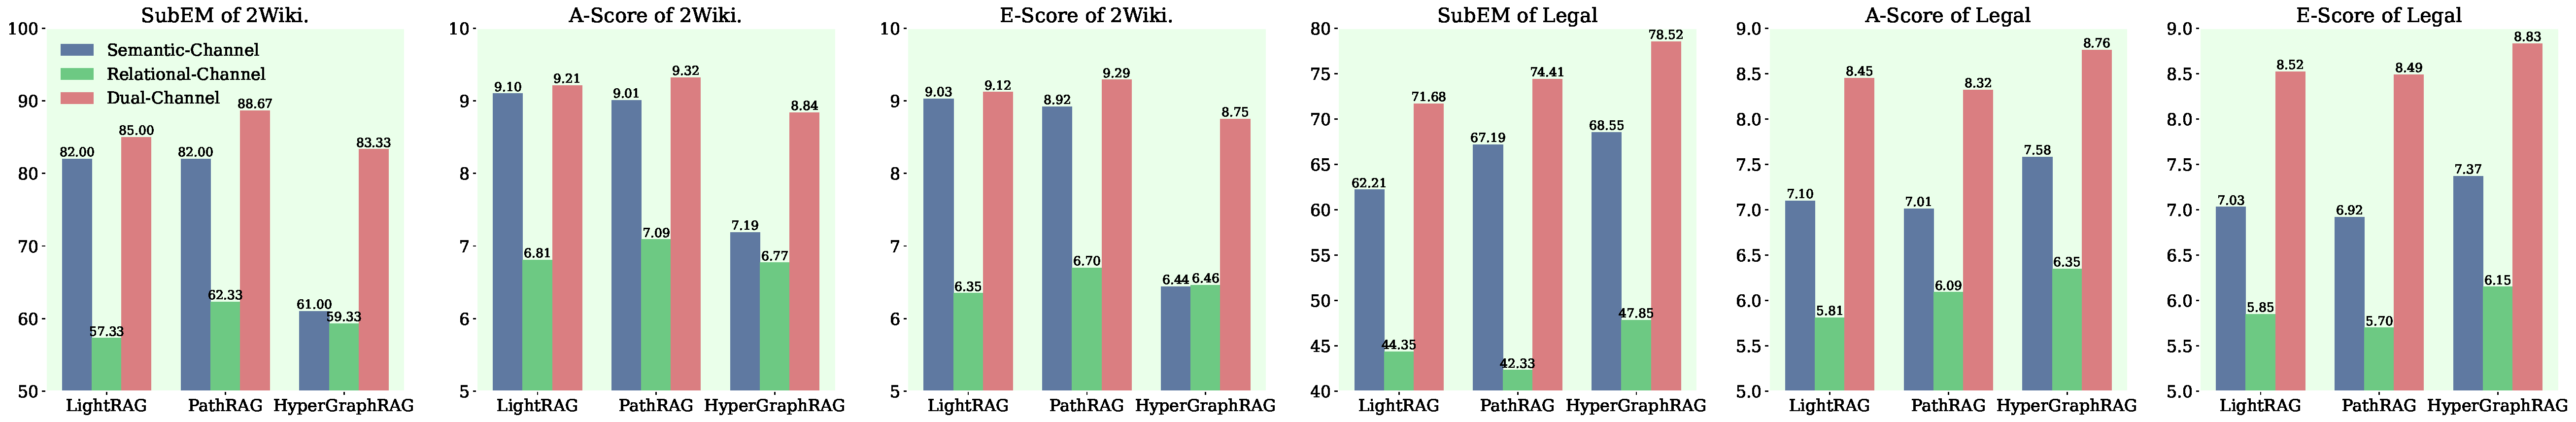
\includegraphics[width=\linewidth]{figs/dual_channel.pdf}
\caption{Comparisons between dual-channel and single-channel retrieval in \textsc{GraphSearch}, integrated with the graph KB retrievers built upon LightRAG, PathRAG and HyperGraphRAG.}
\label{fig:dual_channel}
\vspace{-10pt}
\end{figure}

\begin{table*}[t]
\caption{Experiment results of ablation study across 2Wiki. and Legal datasets of \textsc{GraphSearch} + HyperGraphRAG. \checkmark and / refer to whether each individual module is enable or not.}
\label{Tab:ab_exp}
\setlength{\tabcolsep}{5.5pt}
\begin{center}
\begin{tabular}{ccccccccccccc}
\toprule
\multicolumn{6}{c}{\textbf{Modules}} & 
\multicolumn{3}{c}{\textbf{2Wiki.}} 
& \multicolumn{3}{c}{\textbf{Legal}} \\
\cmidrule[1pt](lr){1-6} \cmidrule[1pt](lr){7-9} \cmidrule[1pt](lr){10-12}
QD & CR & QG & LD & EV & QE 
& {\scriptsize $\mathrm{SubEM}$} & {\scriptsize $\mathrm{A\text{-}Score}$} & {\scriptsize $\mathrm{R\text{-}Score}$}
& {\scriptsize $\mathrm{SubEM}$} & {\scriptsize $\mathrm{A\text{-}Score}$} & {\scriptsize $\mathrm{R\text{-}Score}$} \\
\midrule
\multicolumn{12}{c}{\textbf{\textsc{GraphSearch}} + HyperGraphRAG} \\
\midrule
/ & / & /  & /  & /  & /  
& 64.00 & 7.62 & 7.80 & 66.60 & 8.18 & 8.18 \\
\checkmark & \checkmark & /  & /  & /  & /  
& 76.33 & 8.14 & 8.16 & 73.98 & 8.34 & 8.29 \\
\checkmark & \checkmark & \checkmark & /  & /  & /  
& 81.67 & 8.57 & 8.57 & 77.31 & \textbf{8.82} & 8.71 \\
\checkmark & \checkmark & \checkmark & \checkmark & /  & /  
& 81.33 & 8.66 & \textbf{8.75} & 76.96 & 8.62 & 8.70 \\
\checkmark & \checkmark & \checkmark & \checkmark & \checkmark & \checkmark  
& \textbf{83.33} & \textbf{8.84} & \textbf{8.75} & \textbf{78.52} & 8.76 & \textbf{8.83} \\
\bottomrule
\end{tabular}
\end{center}
\vspace{-10pt}
\end{table*}

\paragraph{\textsc{GraphSearch} modules make clear contributions to the agentic deep searching workflow.}
We empirically evaluate the incremental contributions of the individual components in \textsc{GraphSearch}, including \textit{Query Decomposition (QD)}, \textit{Context Refinement (CR)}, \textit{Query Grounding (QG)}, \textit{Logic Drafting (LD)}, \textit{Evidence Verification (EV)}, and \textit{Query Expansion (QE)}. The design details of each module are provided in Appendix~\ref{app:prompts}. 
\begin{wrapfigure}{r}{0.35\textwidth}
\centering
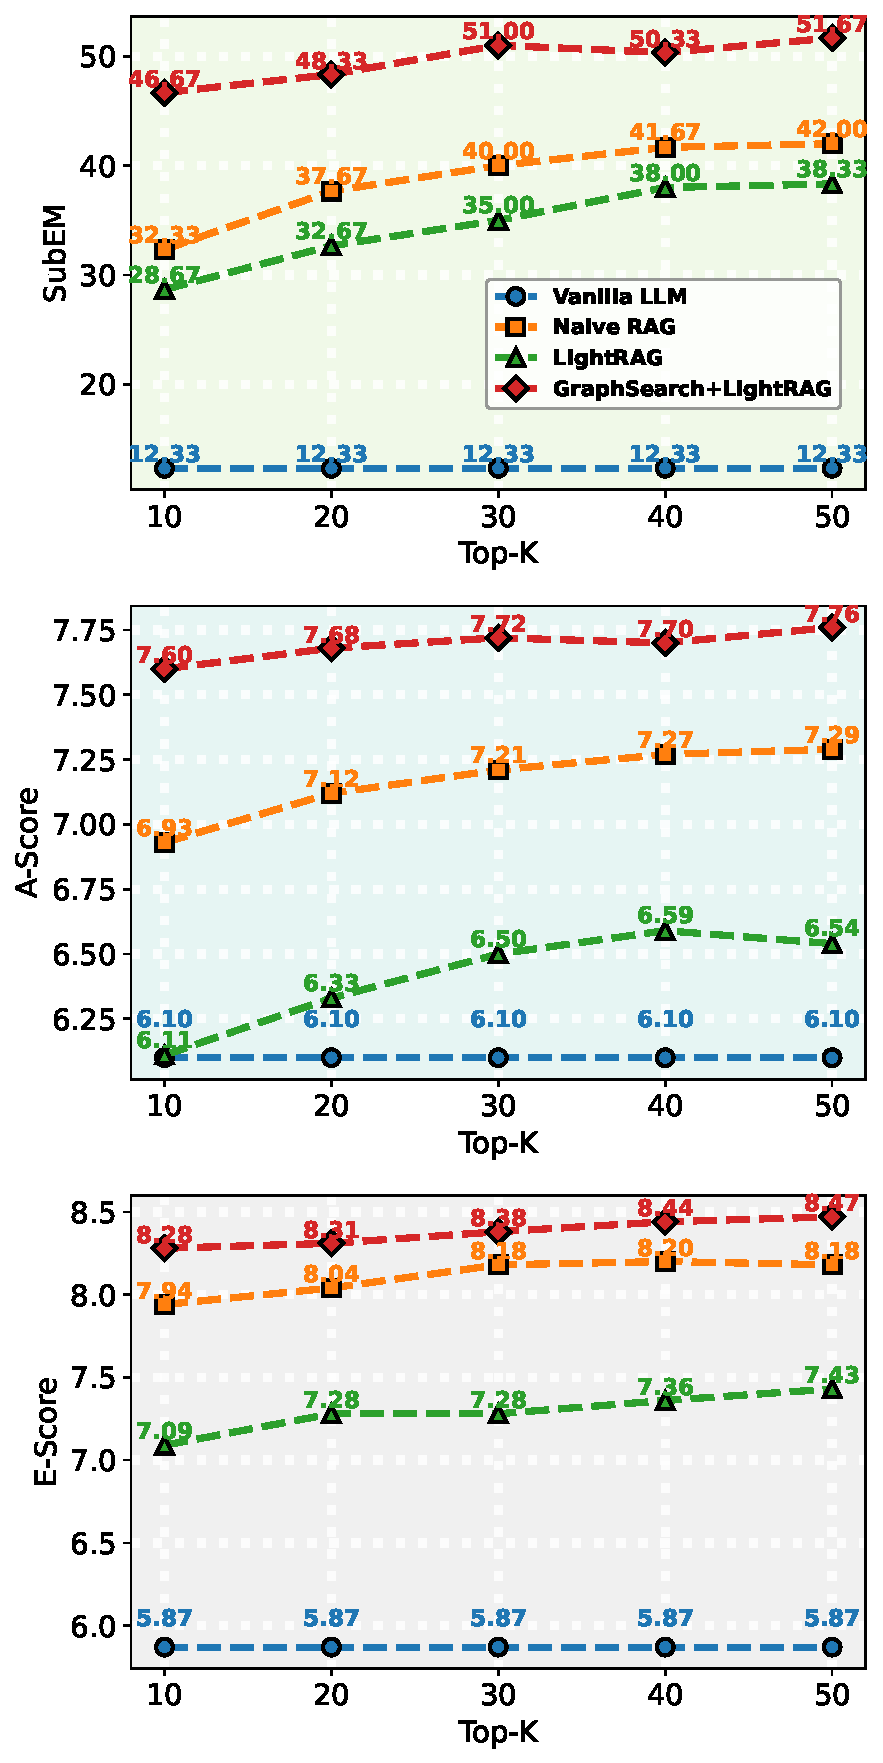
\includegraphics[width=0.35\textwidth]{figs/topk.pdf}
\caption{Performance changes as the count of Top-K varies.}
\label{fig:topk}
\vspace{-30pt}
\end{wrapfigure}
We adopt the graph KB retriever built upon HyperGraphRAG for \textsc{GraphSearch} along with HyperGraphRAG as a baseline. Comparing the combination of [QD, CR] with [QD, CR, QG], the former performs non-iterative question decomposition, producing multiple sub-queries without completing missing information based on retrieved context. Comparing [QD, CR, QG, AD] with the full-module setting, the former only introduces an additional logic drafting, whereas the latter further leverages reflection to generate new sub-queries that fill knowledge gaps. The empirical results confirm the value of the modular orchestration in \textsc{GraphSearch}: from question decomposition, to iterative retrieval, to reflective routing, each step progressively enhances the reasoning process and enables the realization of an agentic deep searching workflow.

\paragraph{\textsc{GraphSearch} exhibits more pronounced advantages under smaller retrieval budgets.} 
By varying the \textbf{Top-K} from $10$ to $50$ as a adjustment strategy for retrieval overhead, the comparison of \textsc{GraphSearch} with baselines on MuSiQue is shown in Figure~\ref{fig:topk}. As Top-K decreases, both Naive RAG and LightRAG show a sharp decline in SubEM and A-Score. In contrast, the drop in E-Score is less pronounced across all three methods, indicating that their retrievers can still capture part of the golden evidence under reduced budgets. However, the absence of critical evidence can prevent models from engaging in sufficient evidence-grounded reasoning, resulting in lower A-Scores relative to the golden answer. By contrast, the agentic searching workflow in \textbf{\textsc{GraphSearch} sustains its performance advantages even under low retrieval overhead}.

\subsection{Further Analysis: Deep Integration of \textsc{GraphSearch} with Graph KBs}

\paragraph{\textsc{GraphSearch} improves the retrieval quality through the dual-channel agentic interaction across both modalities.} 
Using \textbf{Recall} to calculate the golden evidence in the retrieved context, we compare the retrieval quality of \textsc{GraphSearch} with LightRAG, as shown in Figure~\ref{fig:recall}. The \textbf{Step} denotes the interaction rounds performed by \textsc{GraphSearch}, up to the final self-reflection stage. \textsc{GraphSearch} initially retrieves fewer pieces of golden evidence, as it decomposes complex queries into atomic sub-queries. As interactions proceed, the recall of retrieved content shows substantial improvement across both the relational and semantic channels. It confirms that the agentic workflow of \textsc{GraphSearch} is tightly integrated with the features of graph KBs.

\begin{figure}[h]
\centering
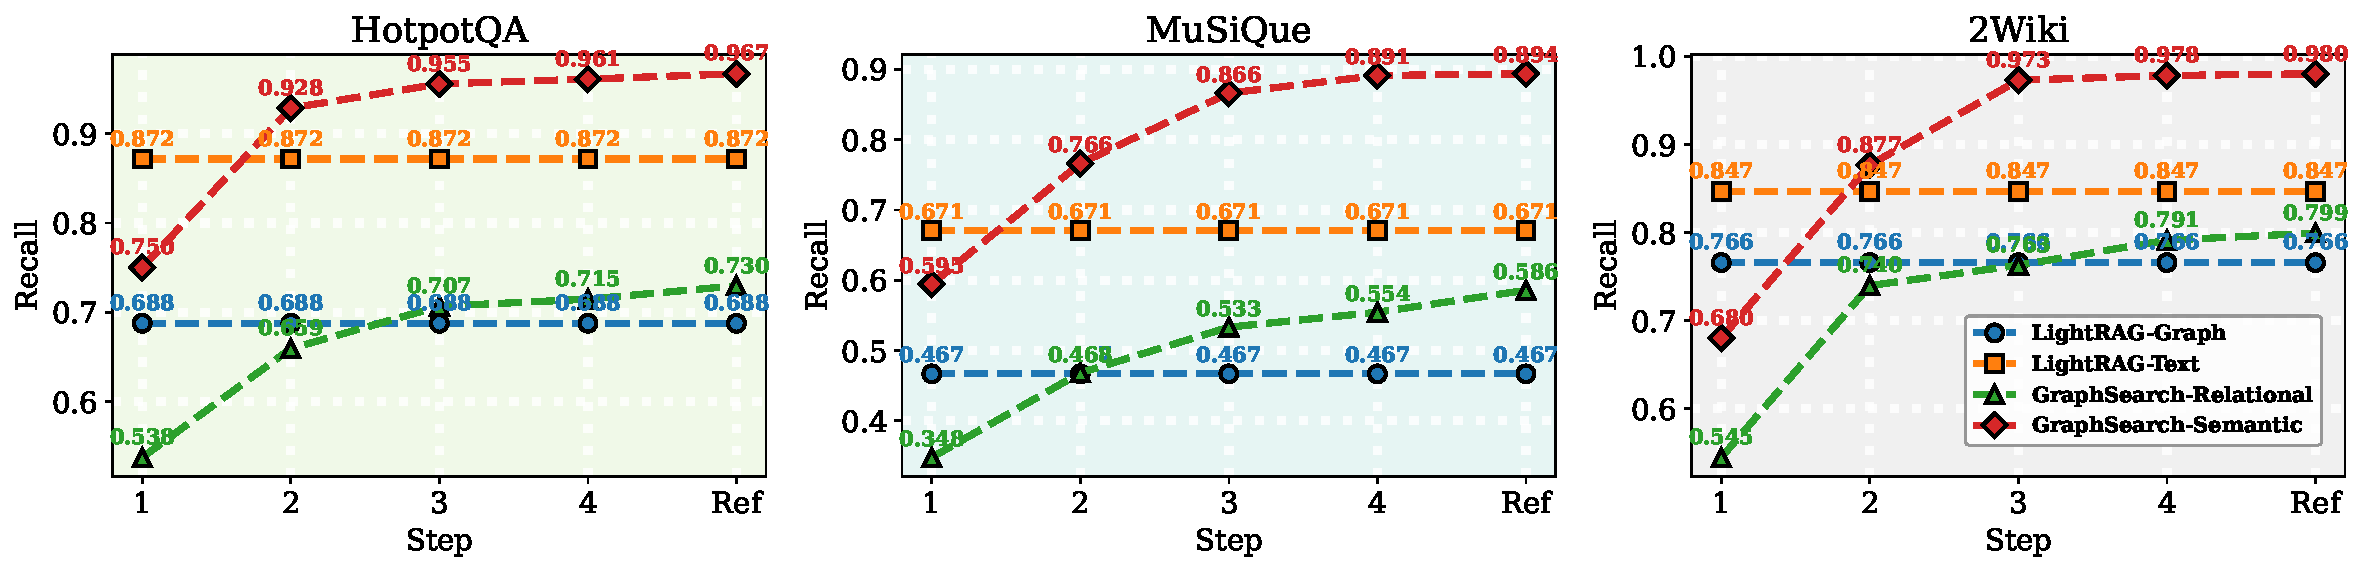
\includegraphics[width=\linewidth]{figs/recall_comparison.pdf}
\caption{\textsc{GraphSearch} improves the recall of golden evidence during agentic interactions.}
\label{fig:recall}
\vspace{-10pt}
\end{figure}

\paragraph{\textsc{GraphSearch} demonstrates a modality–functionality alignment property in dual-channel retrieval.} 
We calculate SubEM on MuSiQue by replacing the retrieval sources of the semantic and relational channel with text and graph data respectively. Results obtained by retrieving from the full data are included as references. Figure~\ref{fig:channel_data} shows that using semantic queries to access text data and relational queries to access graph data consistently outperforms other combinations. Moreover, compared to retrieving from the full data, restricting each channel to its aligned modality not only achieves comparable performance but also substantially reduces context overhead. It confirms that the functionality of the dual-channel retrieval strategy aligns with the data modalities of graph KBs.

\begin{figure}[h]
\centering
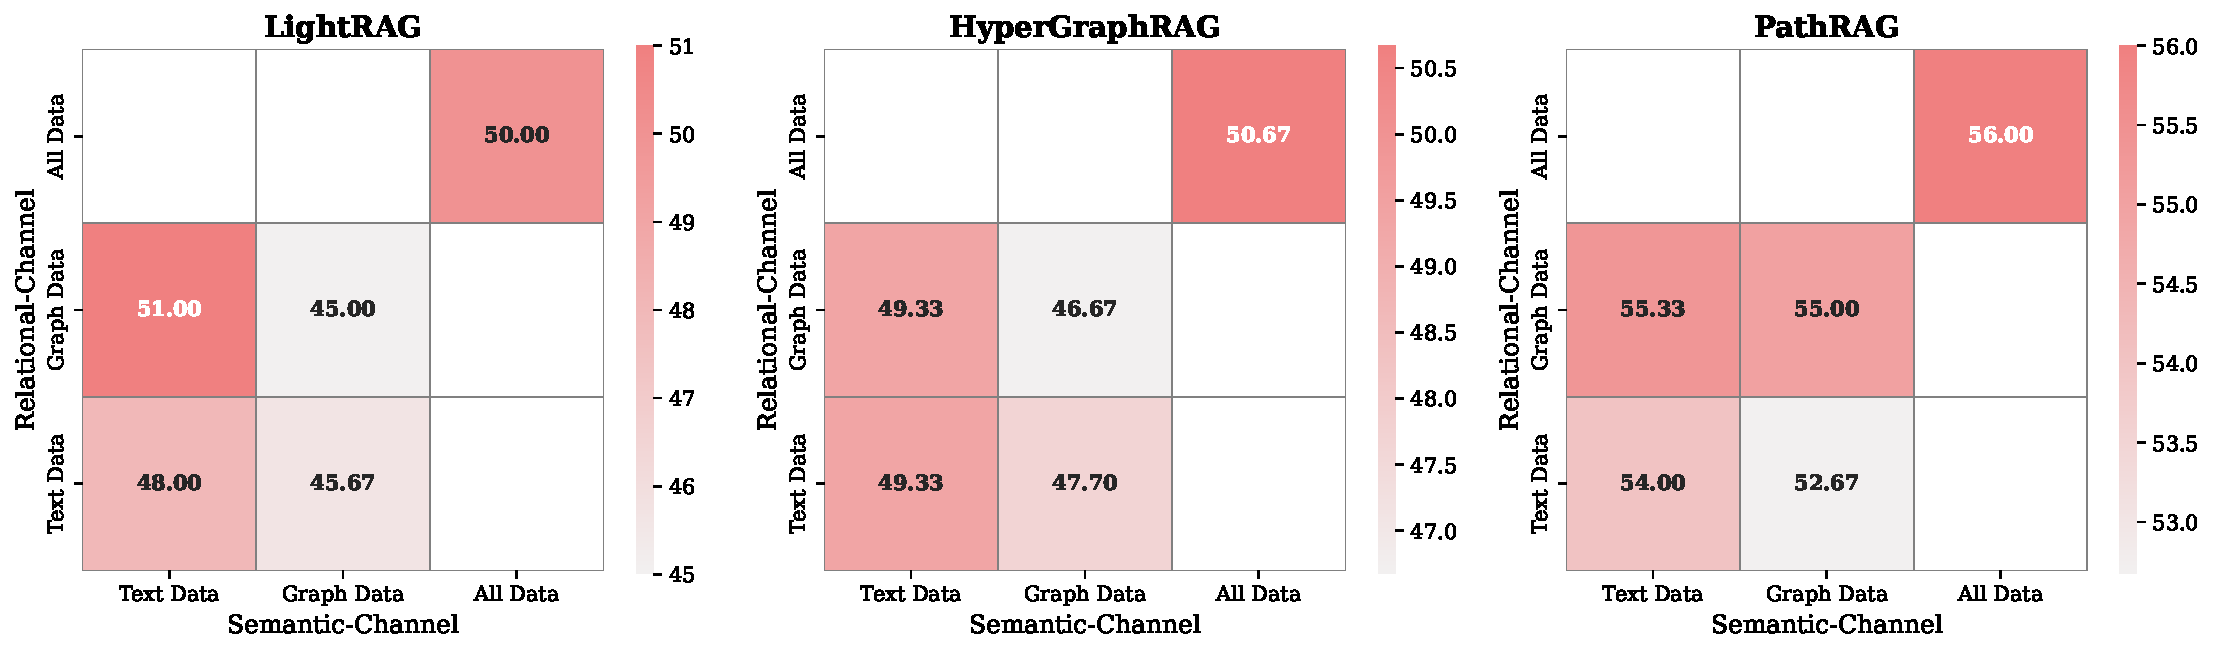
\includegraphics[width=\linewidth]{figs/channel_data.pdf}
\caption{\textsc{GraphSearch} demonstrates a modality–function alignment property.}
\label{fig:channel_data}
\vspace{-10pt}
\end{figure}


% \subsection{Further Analysis: Comparison Between \textsc{GraphSearch} With Agentic RAG}